\documentclass[12pt]{article}
\usepackage{amsmath}
\usepackage{amssymb}
\usepackage[letterpaper,margin=0.85in,centering]{geometry}
\usepackage{fancyhdr}
\usepackage{enumerate}
\usepackage{lastpage}
\usepackage{multicol}
\usepackage{graphicx}

\reversemarginpar

\pagestyle{fancy}
\cfoot{}
\lhead{Math 1560}\chead{Tutorial Assignment \# 6 Solutions}\rhead{May 30th, 2017}
%\rfoot{Total: 10 points}
%\chead{{\bf Name:}}
\newcommand{\points}[1]{\marginpar{\hspace{24pt}[#1]}}
\newcommand{\skipline}{\vspace{12pt}}
%\renewcommand{\headrulewidth}{0in}
\headheight 30pt

\newcommand{\di}{\displaystyle}
\newcommand{\abs}[1]{\lvert #1\rvert}
\newcommand{\len}[1]{\lVert #1\rVert}
\renewcommand{\i}{\mathbf{i}}
\renewcommand{\j}{\mathbf{j}}
\renewcommand{\k}{\mathbf{k}}
\newcommand{\R}{\mathbb{R}}
\newcommand{\aaa}{\mathbf{a}}
\newcommand{\bbb}{\mathbf{b}}
\newcommand{\ccc}{\mathbf{c}}
\newcommand{\dotp}{\boldsymbol{\cdot}}
\newcommand{\bbm}{\begin{bmatrix}}
\newcommand{\ebm}{\end{bmatrix}}      
\usepackage{tikz}
\usetikzlibrary{calc, positioning, decorations.pathmorphing}             
                  
\begin{document}

%\author{Instructor: Sean Fitzpatrick}
\thispagestyle{fancy}
%\noindent{{\bf Name and student number:}}

 \begin{enumerate}
  \item For each of the functions below, use the sign diagram of its derivative to find and classify any critical points.
\begin{enumerate}
 \item $f(x) = 2x^4-4x^2+6$

\bigskip

Since $f'(x) = 8x^3-8x=8x(x^2-1)=8x(x+1)(x-1)$, we get the sign diagram
\begin{center}
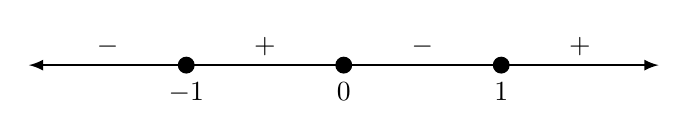
\begin{tikzpicture}[>=latex]
  \draw [thick, <->] (-4,0) -- (4,0);
  \draw [fill] (-2,0) circle [radius =.1];
  \draw [fill] (0,0) circle [radius =.1];
  \draw [fill] (2,0) circle [radius =.1];
  \node at (-3,0) [above] {$-$};
  \node at (-1,0) [above] {$+$};
  \node at (1,0) [above] {$-$};
  \node at (3,0) [above] {$+$};
  \node at (-2,-0.1) [below] {$-1$};
  \node at (0,-0.1) [below] {$0$};
  \node at (2,-0.1) [below] {$1$};
  \end{tikzpicture}
\end{center}

Using the first derivative test, we see that $f$ has a local minimum at $x=-1$, a local maximum at $x=0$, and a local minimum at $x=1$.

\bigskip

 \item $g(x) = \dfrac{x^2}{1+x}$

\bigskip

Since $g'(x) = \dfrac{2x(1+x)-x^2(1)}{(1+x)^2} = \dfrac{x(x+2)}{(x+1)^2}$, we get the sign diagram
\begin{center}
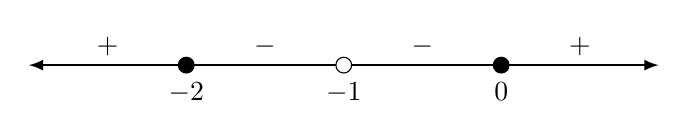
\begin{tikzpicture}[>=latex]
  \draw [thick, <->] (-4,0) -- (4,0);
  \draw [fill] (-2,0) circle [radius =.1];
  \draw [fill=white] (0,0) circle [radius =.1];
  \draw [fill] (2,0) circle [radius =.1];
  \node at (-3,0) [above] {$+$};
  \node at (-1,0) [above] {$-$};
  \node at (1,0) [above] {$-$};
  \node at (3,0) [above] {$+$};
  \node at (-2,-0.1) [below] {$-2$};
  \node at (0,-0.1) [below] {$-1$};
  \node at (2,-0.1) [below] {$0$};
  \end{tikzpicture}
\end{center}
We note that $x=-1$ is not a critical point, since it is not in the domain of $f$. Since $f'$ changes from positive to negative at $x=-2$, this is a local maximum, and since $f'$ changes from negative to positive at $x=0$, this is a local minimum.

\bigskip

 \item $h(x) = x^{7/3}-7x^{1/3}$

\bigskip

We find $h'(x) = \frac{7}{3}x^{4/3}-\frac{7}{3}x^{-2/3} = \frac{7}{3}x^{-2/3}(x^2-1) = \frac{7}{3x^{2/3}}(x-1)(x+1)$. The sign diagram of $h$ is given by
\begin{center}
 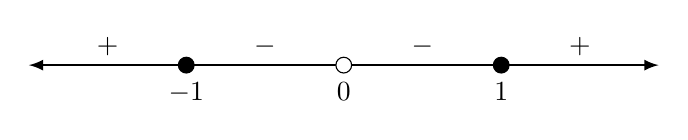
\begin{tikzpicture}[>=latex]
  \draw [thick, <->] (-4,0) -- (4,0);
  \draw [fill] (-2,0) circle [radius =.1];
  \draw [fill=white] (0,0) circle [radius =.1];
  \draw [fill] (2,0) circle [radius =.1];
  \node at (-3,0) [above] {$+$};
  \node at (-1,0) [above] {$-$};
  \node at (1,0) [above] {$-$};
  \node at (3,0) [above] {$+$};
  \node at (-2,-0.1) [below] {$-1$};
  \node at (0,-0.1) [below] {$0$};
  \node at (2,-0.1) [below] {$1$};
  \end{tikzpicture}
\end{center}
We note that although $h'(0)$ is undefined, $h(0)=0$ is defined, so $x=0$ is a critical point. However, it is neither a maximum nor a minimum, since $h'$ has the same sign on both sides of zero. (The graph of $h$ has a vertical tangent at this point.) There are two other critical points: a local maximum at $x=-1$, and a local minimum at $x=1$.
\end{enumerate}

\newpage

 \item For each function below, determine the intervals on which it is increasing/decreasing and concave up/concave down.\\
(Note: these are the same functions as in the previous problem.)

\begin{enumerate}
 \item $f(x) = 2x^4-4x^2+6$

\bigskip

The intervals of increase and decrease can be obtained directly from the sign diagrams in the previous problem. Since $f$ is increasing wherever $f'(x)>0$, we see that $f$ is increasing on $(-1,0)\cup (1,\infty)$, and similarly, $f$ is decreasing wherever $f'(x)<0$, which is on $(-\infty,-1)\cup (0,1)$.

For concavity, we compute $f''(x) = 24x^2-8 = 8(3x^2-1) = 8(\sqrt{3}x-1)(\sqrt{3}x+1)$, so $f''(x)=0$ when $x=\pm \dfrac{1}{\sqrt{3}}$. The sign diagram for $f''$ is
\begin{center}
 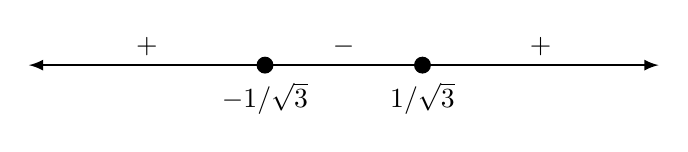
\begin{tikzpicture}[>=latex]
  \draw [thick, <->] (-4,0) -- (4,0);
  \draw [fill] (-1,0) circle [radius =.1];
   \draw [fill] (1,0) circle [radius =.1];
  \node at (-2.5,0) [above] {$+$};
  \node at (0,0) [above] {$-$};
  \node at (2.5,0) [above] {$+$};
  \node at (-1,-0.1) [below] {$-1/\sqrt{3}$};
  \node at (1,-0.1) [below] {$1/\sqrt{3}$};
  \end{tikzpicture}
\end{center}

From the sign diagram, we see that $f$ is concave up for $x\in (-\infty,-1/\sqrt{3})\cup (1/\sqrt{3},\infty)$, and concave down on $(-1/\sqrt{3},1/\sqrt{3})$.

\bigskip


 \item $g(x) = \dfrac{x^2}{1+x}$

\bigskip

 From the sign diagram for $g'$, we see that $g$ is increasing on $(-\infty, -2)\cup(0,\infty)$, and decreasing on $(-2,-1,)\cup (-1,0)$. (Note that we must exclude $x=-1$ from the interval of decrease, since there is a vertical asymptote there.)

 The second derivative is given by
\[
 g''(x) = \frac{d}{dx}\left(\frac{x^2+2x}{(x+1)^2}\right) = \frac{(2x+2)(x+1)^2-(x^2+2x)(2(x+1))}{(x+1)^4} = \frac{2}{(x+1)^3}
\]
 We see that $g''$ is undefined at $x=-1$ (the vertical asymptote), and $g''(x)>0$ (so $g$ is concave up) on $(-1,\infty)$, while $g''(x)<0$ (so $g$ is concave down) on $(-\infty, -1)$.

\bigskip


 \item $h(x) = x^{7/3}-7x^{1/3}$

\bigskip

 The sign diagram for $h'$ shows that $h$ is increasing on $(-\infty, -1)\cup (1,\infty)$ and decreasing on $(-1,1)$. (Note that $h$ is defined at $x=0$, even if $h'$ is not. It's a fairly arbitrary choice as to whether or not to include 0 here.) For concavity, we compute
\[
 h''(x) = \frac{d}{dx}\left(\frac{7}{3}x^{4/3}-\frac{7}{3}x^{-2/3}\right) = \frac{28}{9}x^{1/3}+\frac{14}{9}x^{-5/3} = \frac{14}{9x^{5/3}}(x^2+1).
\]
We see that $h''(x)$ is undefined at $x=0$ and that $h''$ has no zeros. We can conclude that the graph of $h$ is concave up for $x>0$, and concave down for $x<0$.
\end{enumerate}

\end{enumerate}


\end{document}